\section{Results}\label{sec:results}

Muons and beam-related background  were generated by the 11 GeV electron beam interaction with the beam-dump and propagated in the region of interest as described in  Sec.~\ref{sec:sampling}. 

\begin{figure}[h!] 
\center
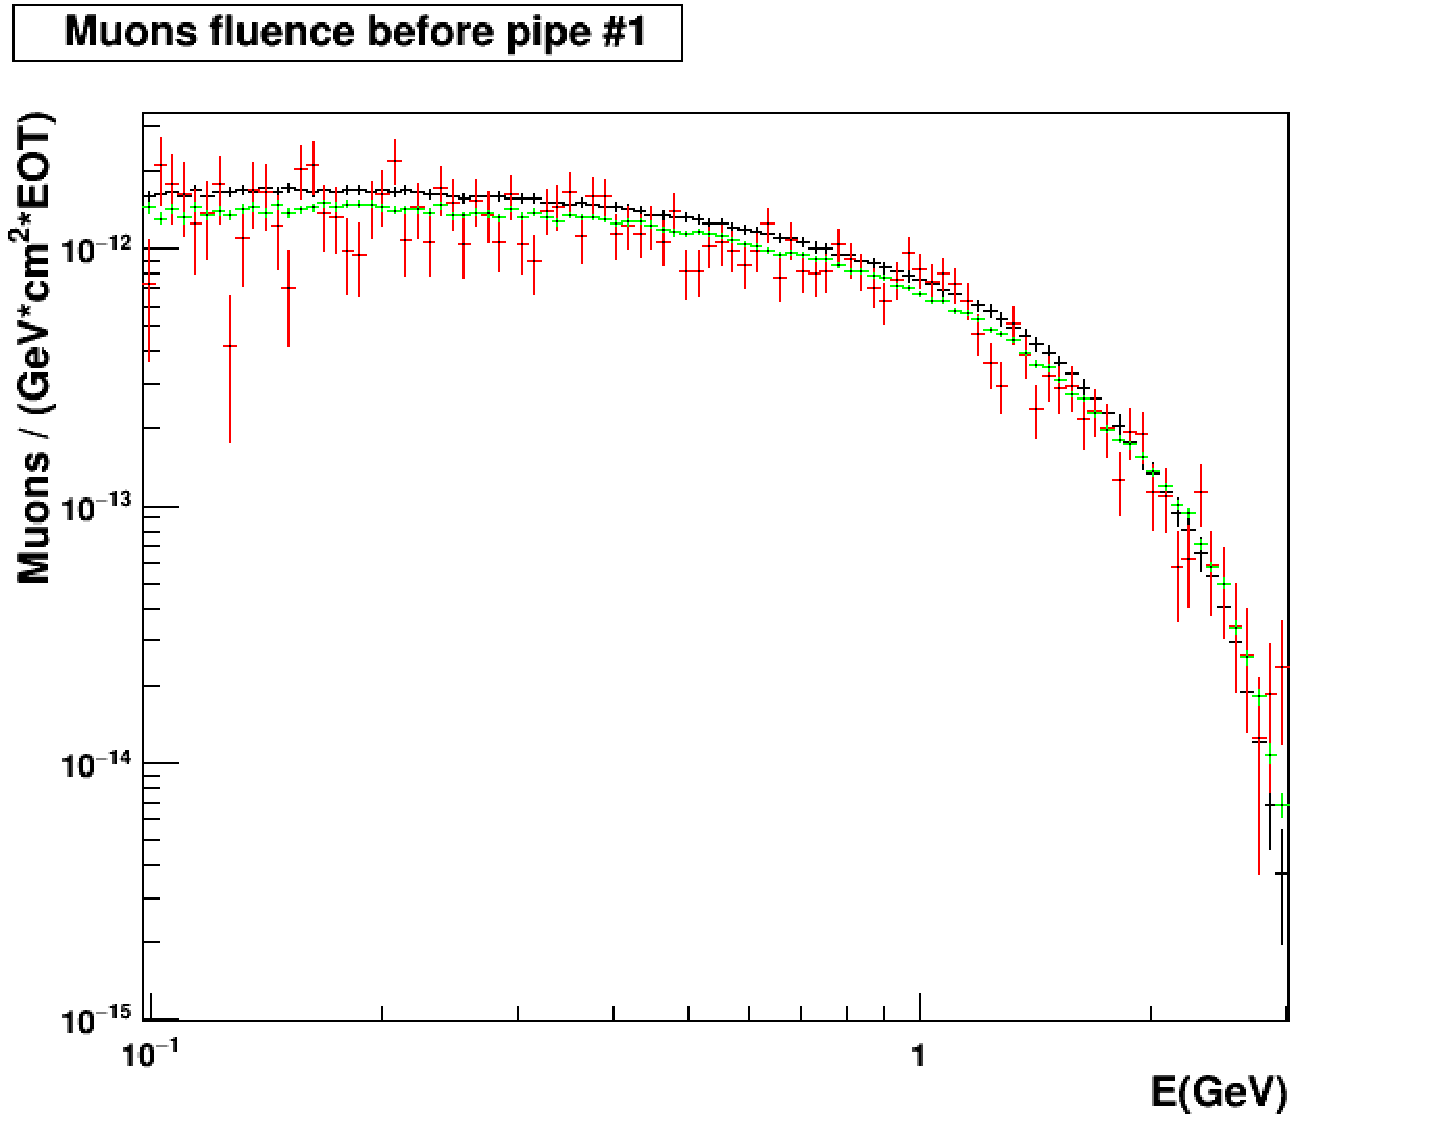
\includegraphics[width=4.7cm]{figs/comparisonMuonsPipe1_1D.pdf}
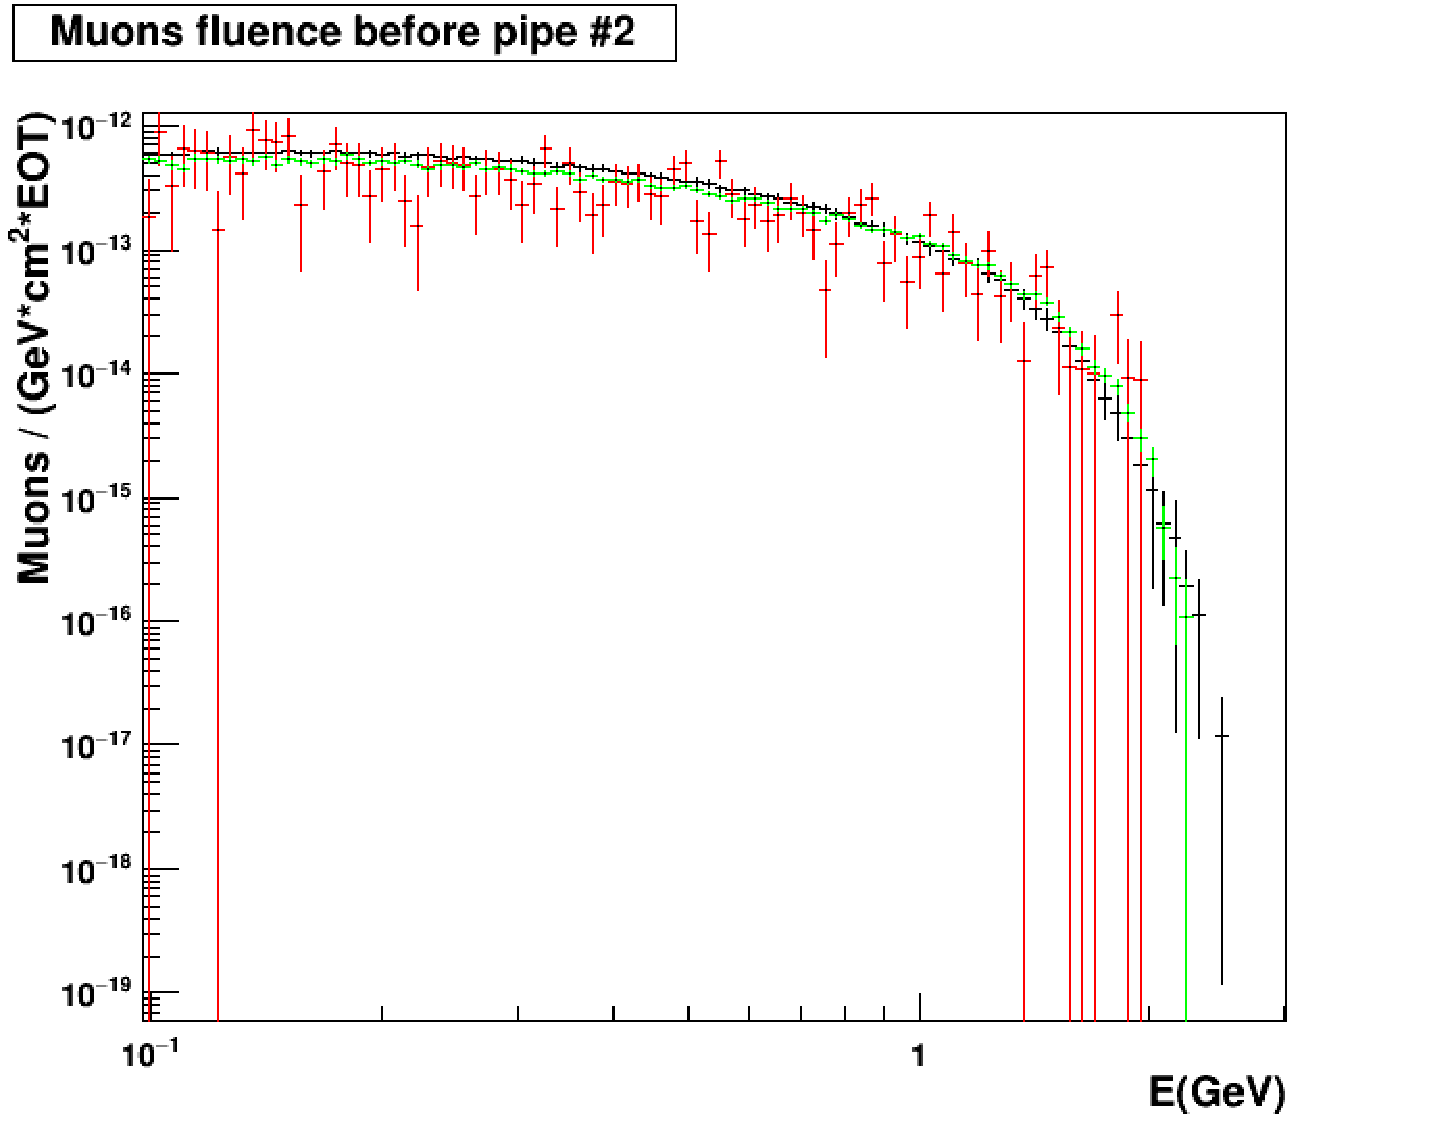
\includegraphics[width=4.7cm]{figs/comparisonMuonsPipe2_1D.pdf}
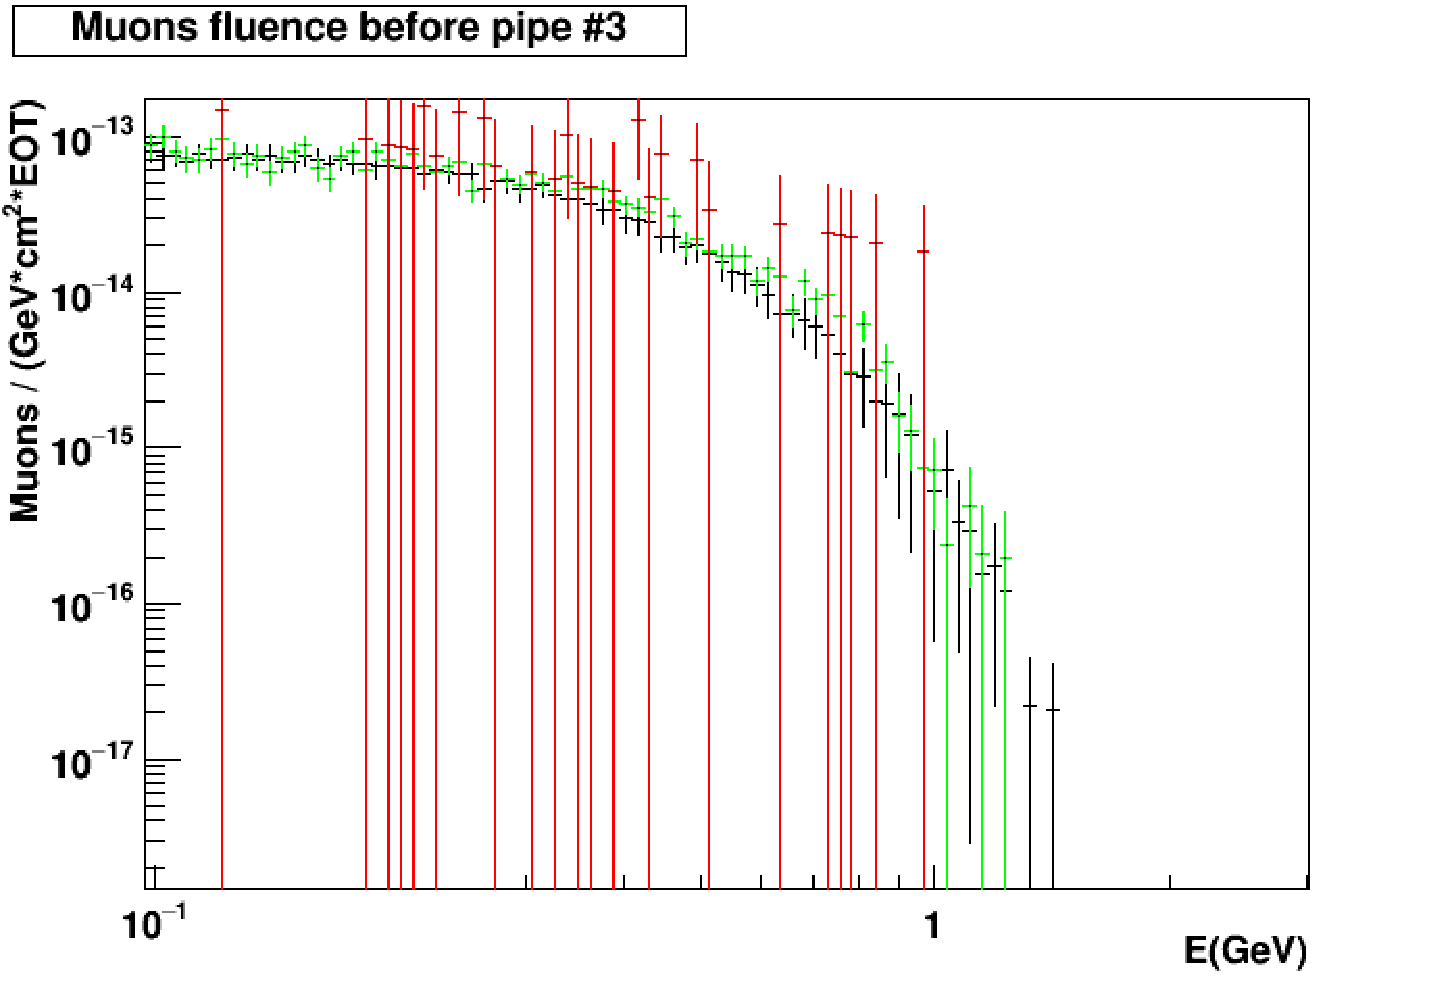
\includegraphics[width=5.5cm]{figs/comparisonMuonsPipe3_1D.pdf}
\caption{Muons differential fluence at the three locations of interest (A, B and C). Beam/dump interaction using  FLUKA (black), GEMC (red) and the high statistic custom $\mu$ event generator with GEMC propagation (green).}
\label{fig:mu-comp}
\end{figure}


\subsection{Muon detection} 
Fig.~\ref{fig:mu-comp} shows the muon flux crossing the BDX-Hodo  as obtained by GEMC and FLUKA  in the  three locations of interest ({\bf A}, {\bf B} and {\bf C}).
The flux has been sampled assuming the BDX-Hodo centered to  the beam-line depth.
Results are reported for muons generated at high statistic by the custom $\mu$ event generator and propagated using GEMC (green points in the figure).
The number of event generated at the dump correspond to  (1.2 $\pm$0.1) 10$^{12}$ EOT or one second of 0.2 $\mu$A current.
Rates in crystal, scintillators and  requiring a 5-fold coincidence of the two front/back layers of plastic with  the crystal are reported in Tab.~\ref{tab:rate} for a beam current of 10$\mu$A and detection thresholds as listed in the previous Section. Results show a drop in rate by about one order of magnitude when moving from one location to the next. 
Table~\ref{tab:rate-height}  shows the expected rate measured in  position {\bf C}  when the BDX-Hodo detector is off-axes by 40/80 cm. The measurement of muon rate at different heights (angles) wrt to the beam-line (beam-dump) will provide further information to validate simulations.  
Fluxes in position {\bf C} (or/and {\bf B}) are large enough to be detectable (significantly higher than cosmic muons and beam-dump neutron background) and manageable  by crystal, SiPms and front-end electronics (no pile-up effects expected). These two locations are close to the paved road and easily accessible by the drilling machine and related equipment. Similar conclusions (scaling rates by 10) hold  if the beam current drops/increases by one order of magnitude (1/100 $\mu$A) making the test feasible in parallel to any 11 GeV operation of Hall-A.

\begin{table}[htp]
\caption{Beam-on muon rates expected in BDX-Hodo for I$_{beam}$=10$\mu A$ in locations {\bf A}, {\bf B},  and {\bf C}.}
\begin{center}
\begin{tabular}{|c|c|c|c|c|}
\hline
Location & Rate$_{Crystal}$  (kHz)&  Rate$_{Front-Back \;Scint} $(kHz) & Rate$_{Coin}$ (kHz) & Rate$_{XY\, ch} $(kHz)\\
\hline\hline
{\bf A}  & 120  &120/40    & 24 &4.5 \\
 \hline
{\bf B} & 20 &  22/8 & 3.7 & 0.7\\
 \hline
{\bf C} & 2.8 &  2.5/1 & 0.5 & 0.1 \\
\hline\hline
\end{tabular}
\end{center}
\label{tab:rate}
\end{table}%

\begin{table}[htp]
\caption{Beam-on muon rates expected in BDX-Hodo for I$_{beam}$=10$\mu A$ in position {\bf C} sampled at different vertical distance from the beam-line.}
\begin{center}
\begin{tabular}{|c|c|c|c|c|}
\hline
Vertical distance  & Rate$_{Crystal}$  (kHz)&  Rate$_{Front-Back \;Scint} $(kHz) & Rate$_{Coin}$ (kHz) & Rate$_{XY\, ch} $(kHz)\\
\hline\hline
0 (nominal)  & 2.8  &2.5/1    & 0.5 &0.1 \\
 \hline
40 cm & 1.4 &  2.5/1.5 & 0.17 & 0.04 \\
 \hline
80 cm&  0.6  & 0.6/0.3    &  0.08 & 0.02 \\
\hline\hline
\end{tabular}
\end{center}
\label{tab:rate-height}
\end{table}


\subsection{Muon flux above-the-ground}
For sake of completeness the muon flux has also been evaluated by using FLUKA in the closest locations accessible above the  beam-dump vault .  This set-up assumes to locate the detector above-the-ground with no drilling required  largely  simplifying the test.
Due to the CPU-time necessary to track muons at such large angle (with respect to the beam axis) we used a two steps procedure. Firstly, the 11 GeV electron beam was let to interact with the beam-dump and muons produced on the roof of the vault sampled in four  different locations (shown in  Fig.~\ref{fig:bd-top}-left ).
A high statistic sample of muons have then been generated according to the previous distributions and propagated to the outside.  Applying  a conservative hypothesis (the muons are propagated perpendicular to the beam axis  crossing the minimal amount of concrete and dirt) muons with energy higher than 4.5 GeV (the minimum to not been ranged out)  were propagated and sampled in the four  perpendicular outdoor positions. Figure~\ref{fig:bd-top}-right shows the four locations (A$_{Ext}$, B$_{Ext}$, C$_{Ext}$,  and D$_{Ext}$) on top of the hill. Integrating  over the surface of the BDX-Hodo detector ($\sim 100$ cm$^2$) and considering as a reference a beam current of 10 $\mu$A, no sizeable muon flux would be detected (Rate$_{Max}<$3 Hz). Rates in the different outdoor locations are listed in Tab.~\ref{tab:outside}.

\begin{figure}[h!] 
\center
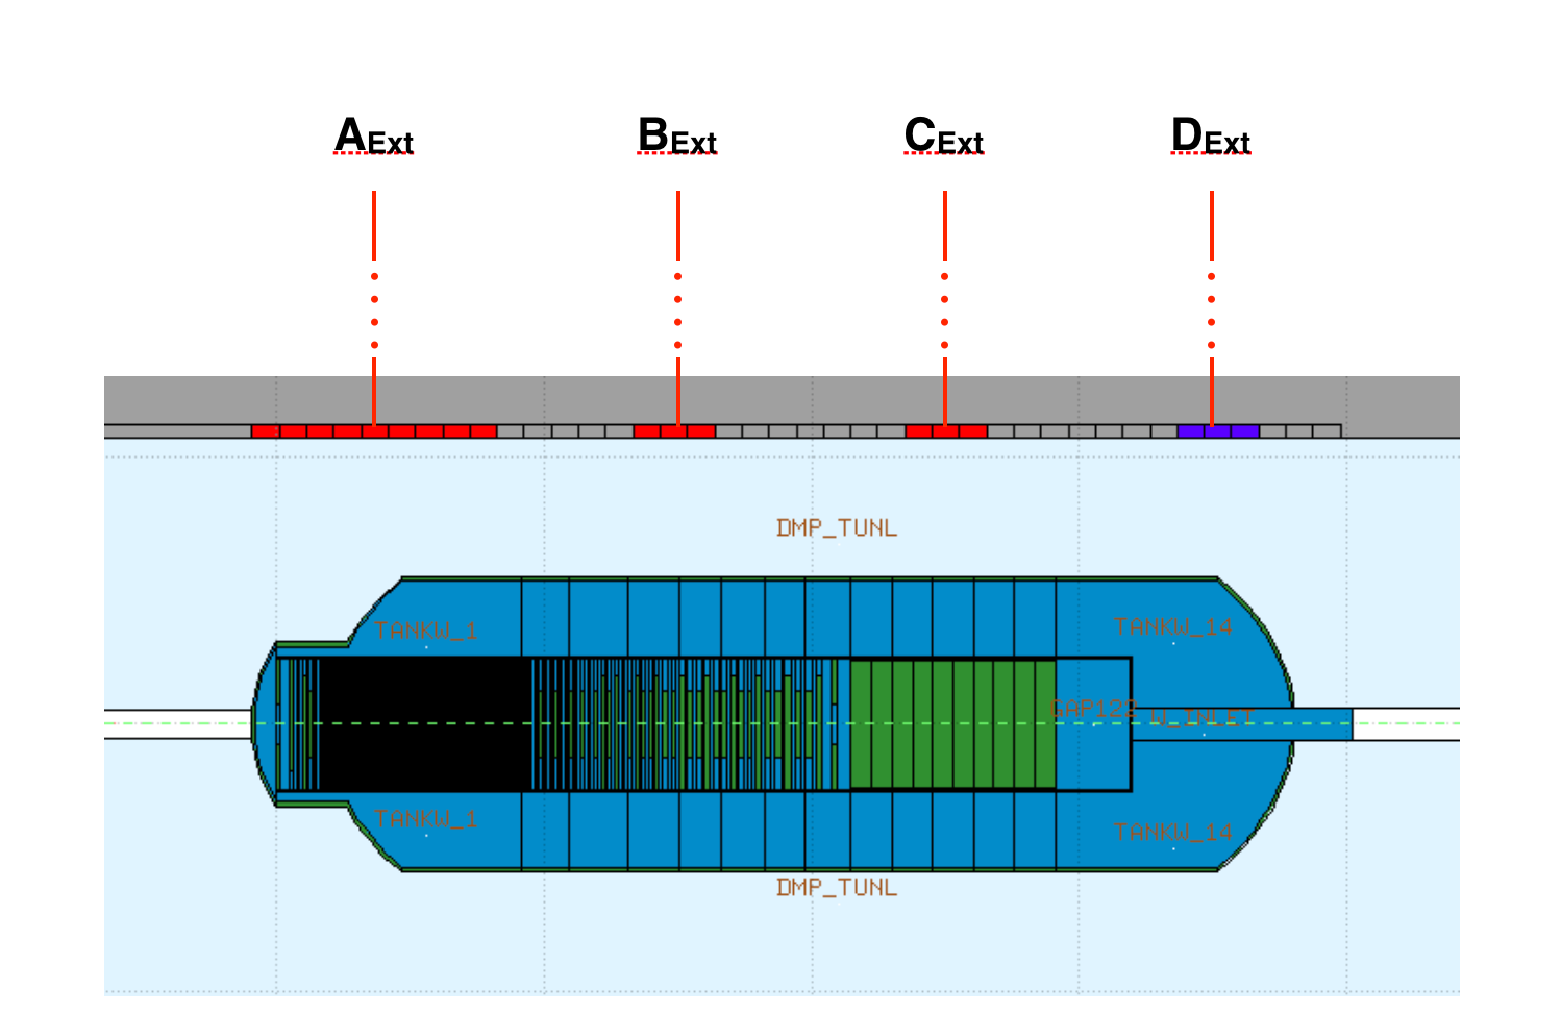
\includegraphics[width=8.0cm]{figs/DumpTunnelTopBigger1.pdf}
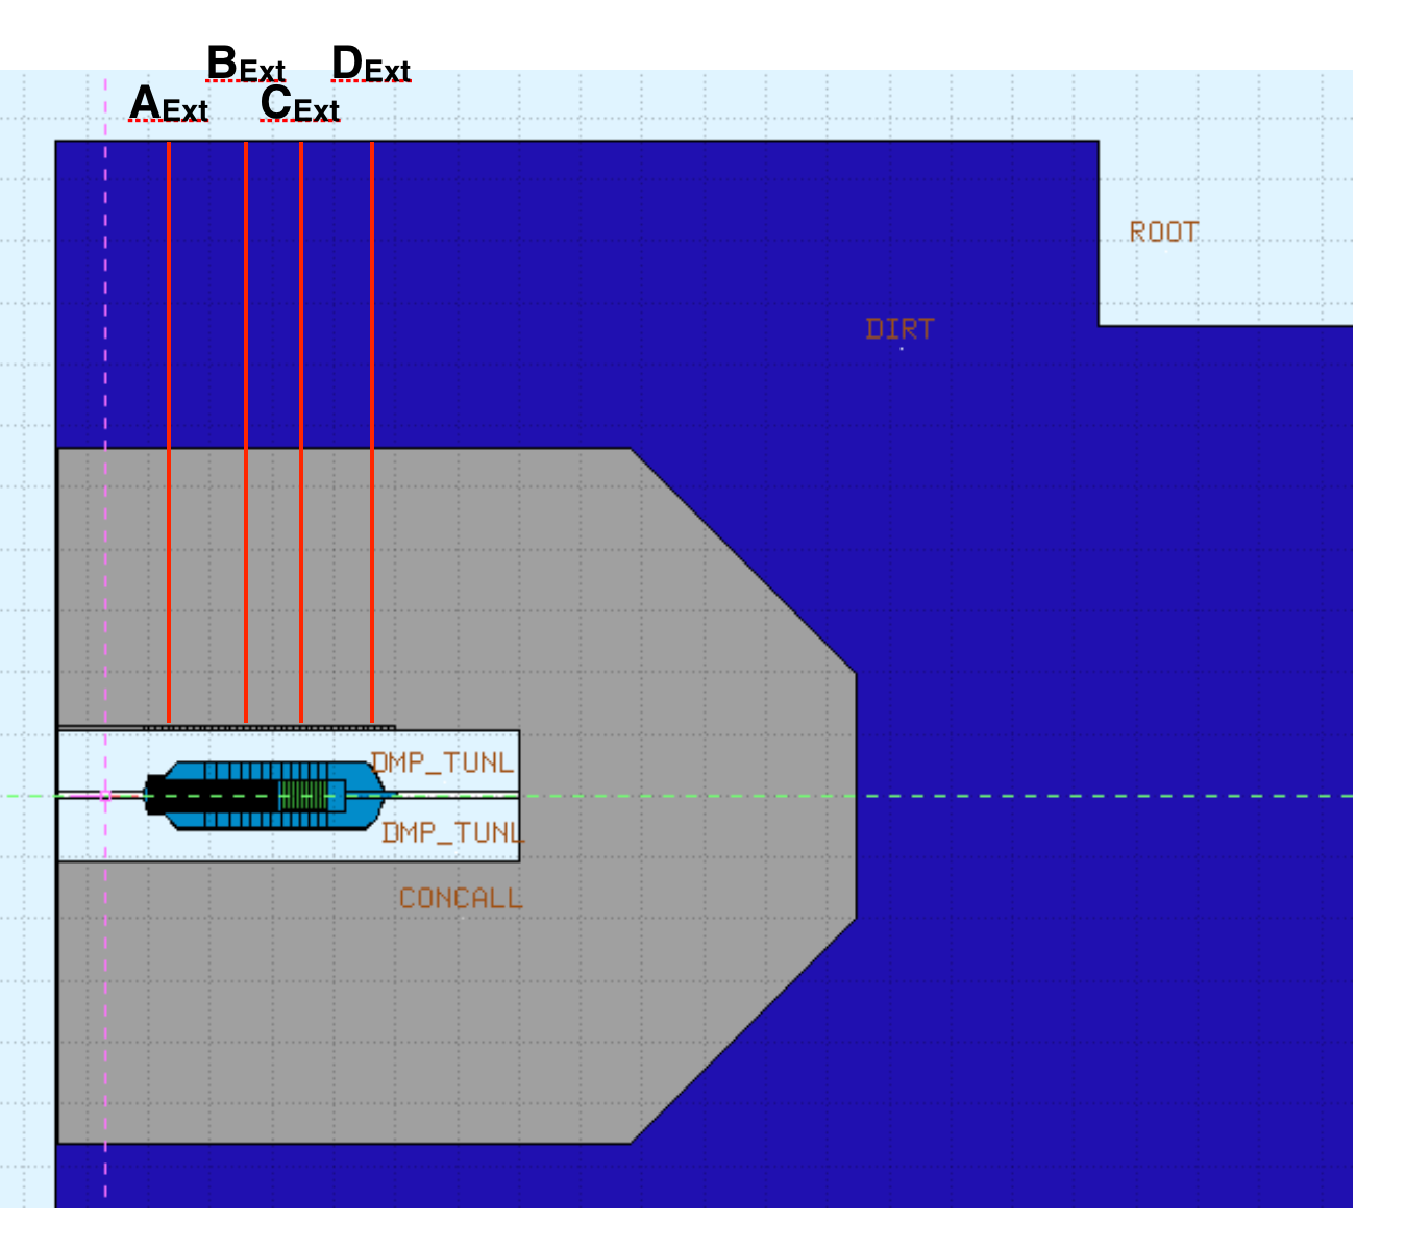
\includegraphics[width=5.7cm]{figs/DumpTunnelTop1.pdf}
\caption {Left: In red are shown the points on the roof  where muon flux has been sampled. Right:  A$_{Ext}$, B$_{Ext}$, C$_{Ext}$,  and D$_{Ext}$ are the four location outdoor where the muon flux has been evaluated.}
\label{fig:bd-top}
\end{figure}


\begin{table}[htp]
\caption{Beam-on muon rate expected outdoor,  on top of the beam-dump hill.}
\begin{center}
\begin{tabular}{|c|c|}
\hline
Location &Rate$_{Crystal} $ (Hz / (cm$^2$ $\mu$A) \\
\hline\hline
A$_{Ext} $ & 2.2 $10^{-3}$\\
 \hline
B$_{Ext} $ & 4.7 $10^{-4}$\\
 \hline
C$_{Ext} $ & 1.9 $10^{-3}$\\
 \hline
D$_{Ext}$ & negligible\\

\hline\hline
\end{tabular}
\end{center}
\label{tab:outside}
\end{table}




\subsubsection{Beam-related background}
Beside muons, other particles are produced in the 11 GeV electron beam interaction with the dump.
The majority (electrons, gamma, nuclei and fragments) are ranged-out well before to reach the region of interest but some (low energy neutrons, mainly) may propagate through  concrete and  dirt reaching the BDX-Hodo detector.
Fig.~\ref{fig:nu-comp} shows the neutron flux  in the  three locations of interest as obtained by  FLUKA simulations. 
\begin{figure}[h!] 
\center
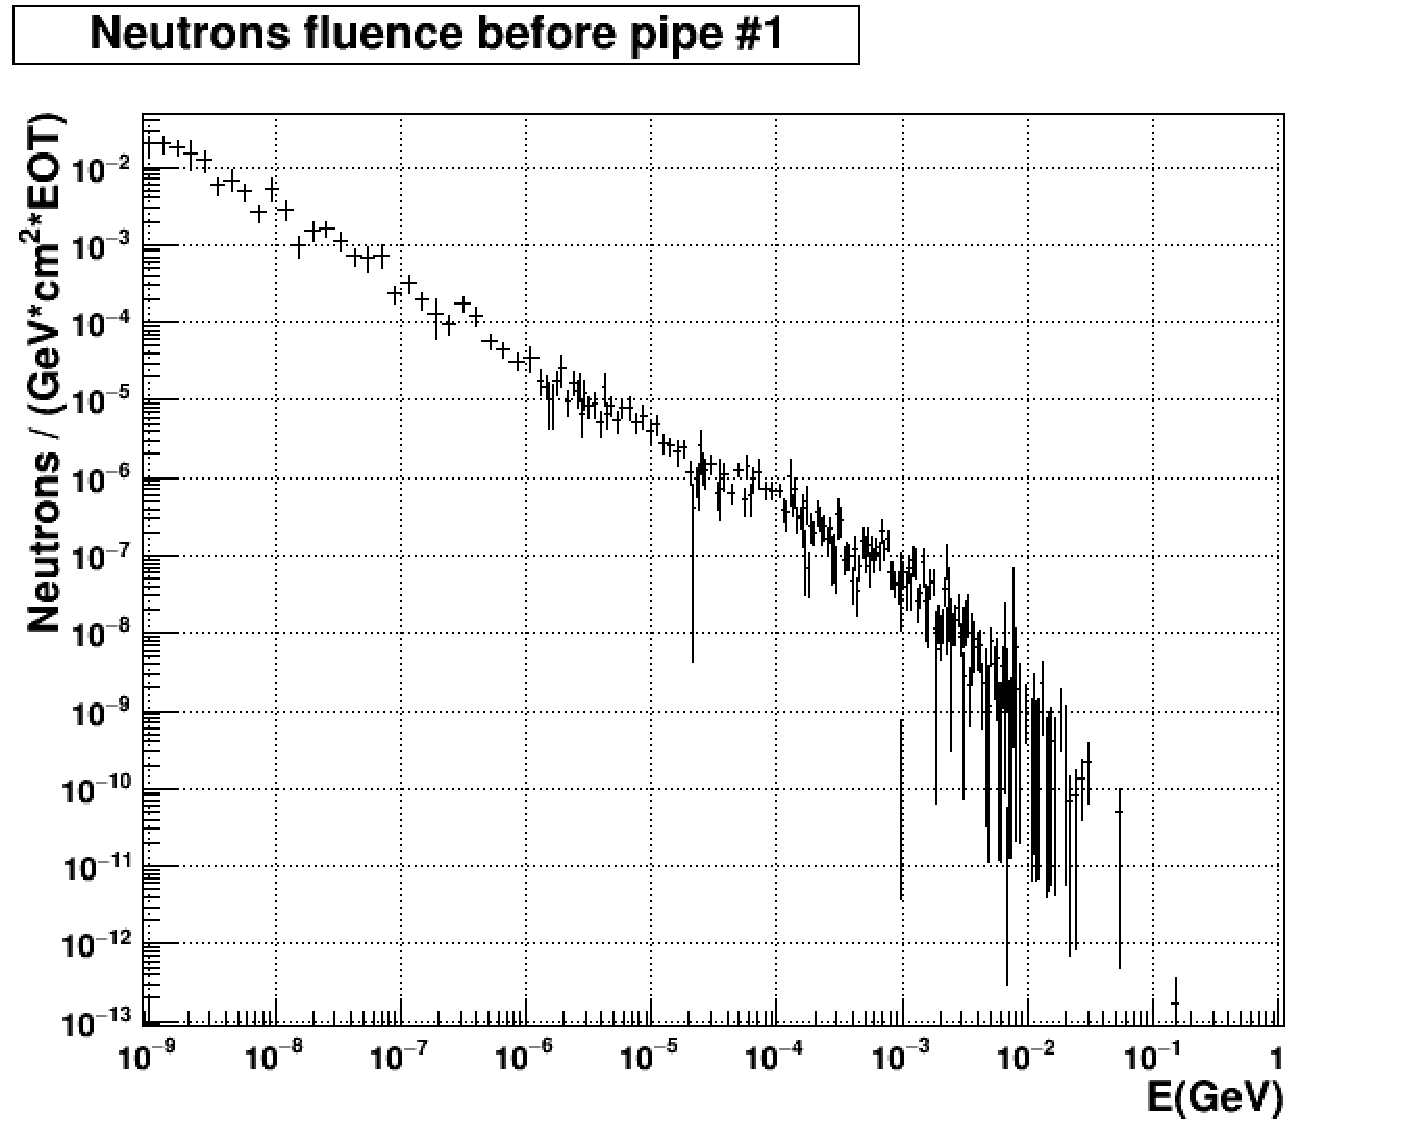
\includegraphics[width=4.9cm]{figs/NeutronsPipe1_1D.pdf}
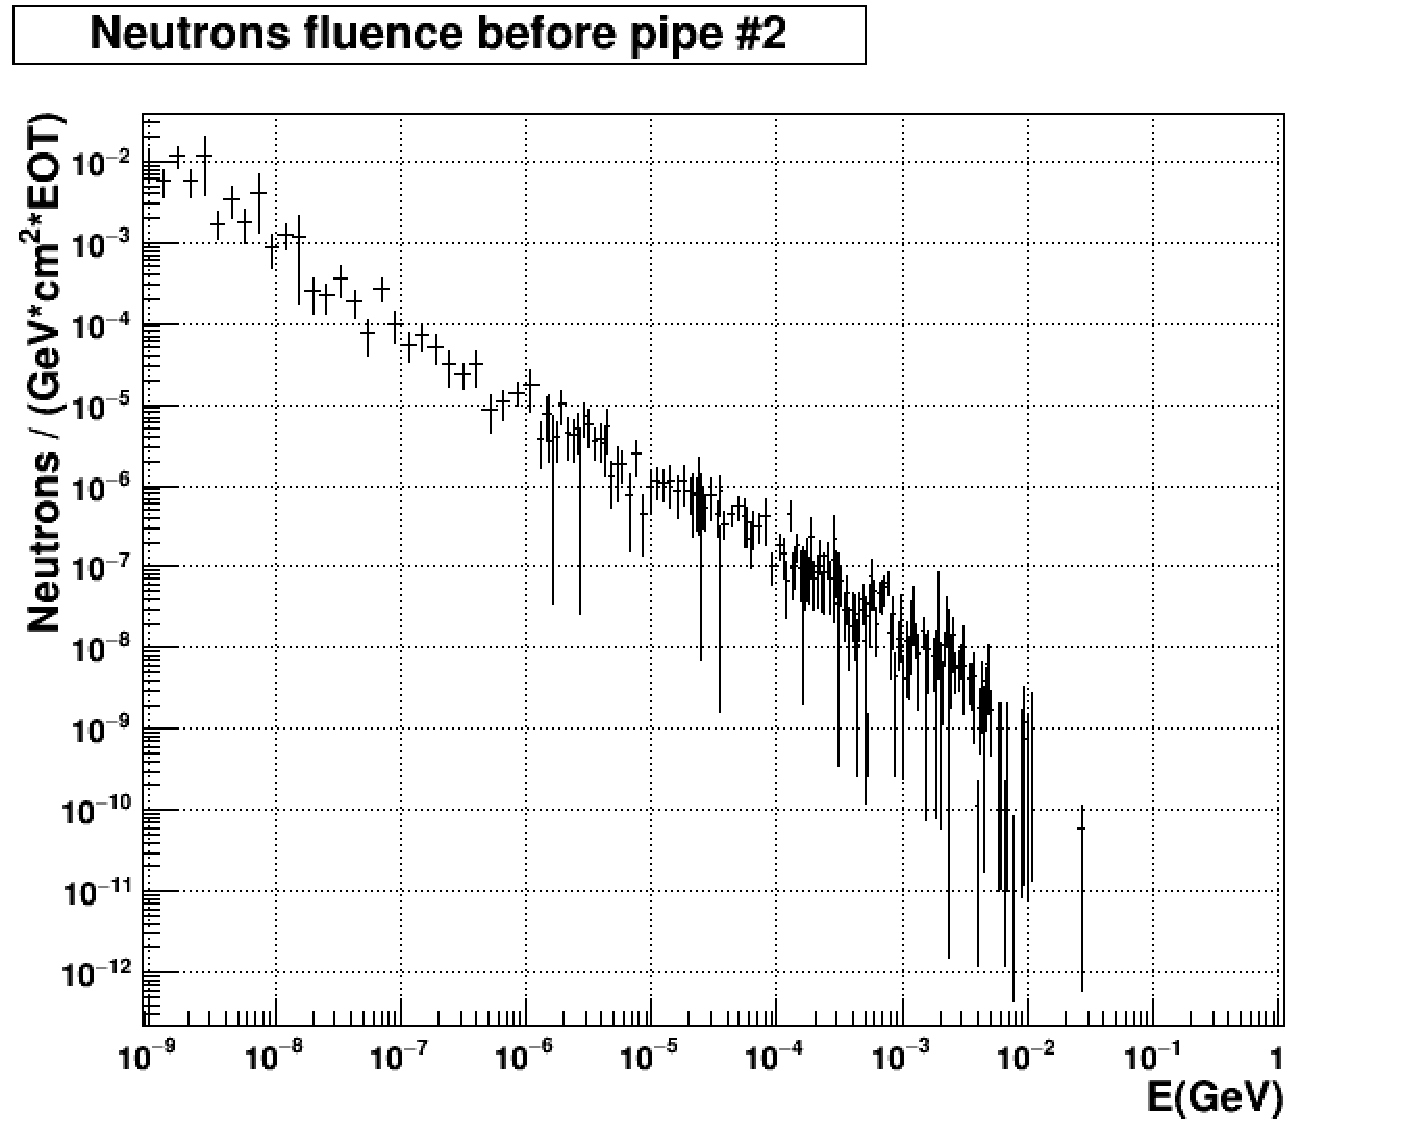
\includegraphics[width=4.9cm]{figs/NeutronsPipe2_1D.pdf}
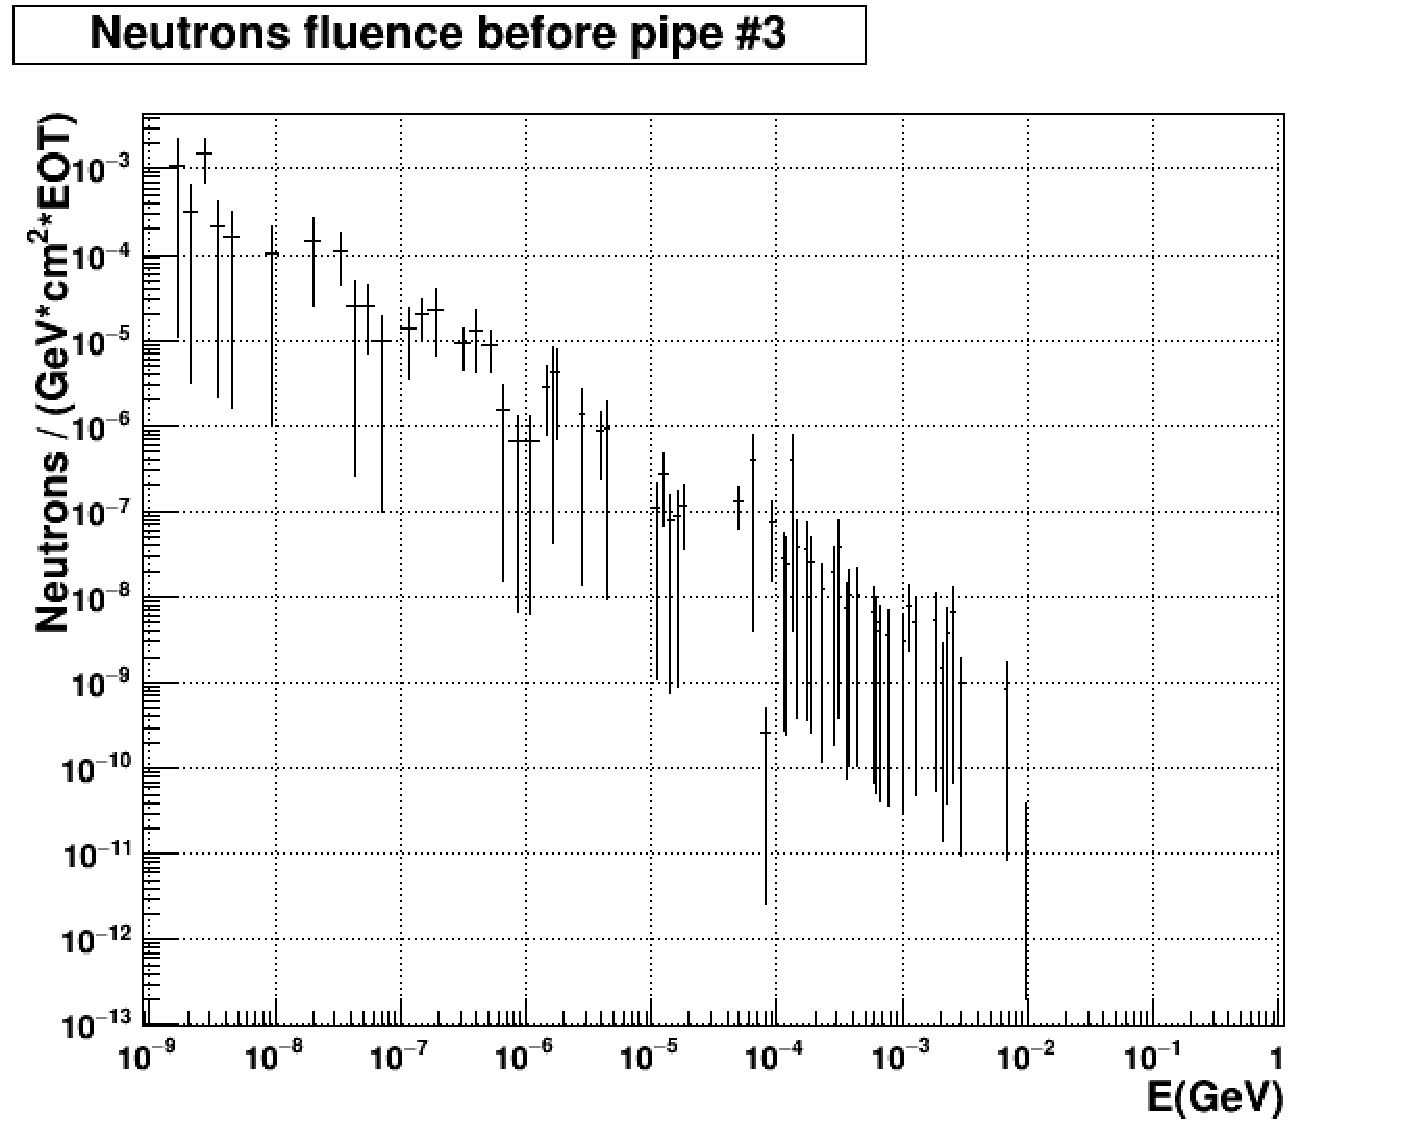
\includegraphics[width=4.9cm]{figs/NeutronsPipe3_1D.pdf}
\caption {Neutron differential fluence at the three locations of interest. Spectra are obtained from electron beam interaction with the beam-dump using FLUKA.}
\label{fig:nu-comp}
\end{figure}
\begin{figure}[h!] 
\center
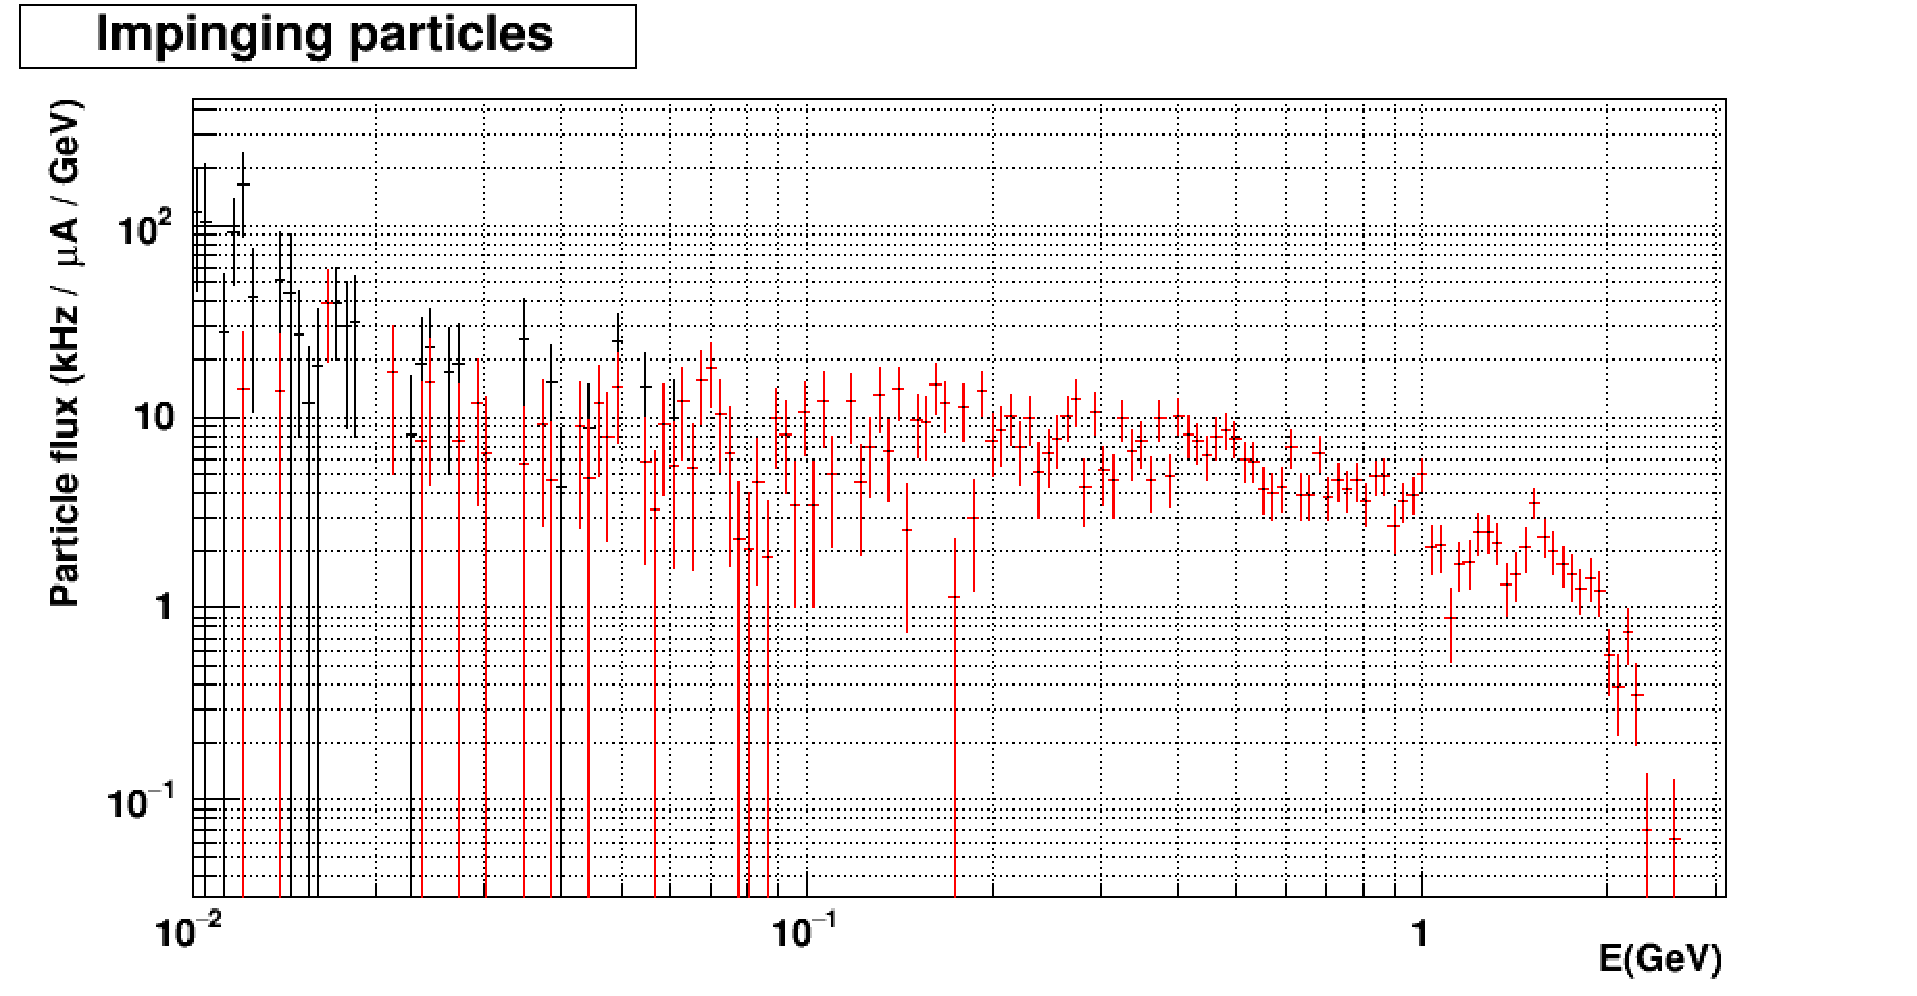
\includegraphics[width=10.0cm]{figs/fig10.pdf}
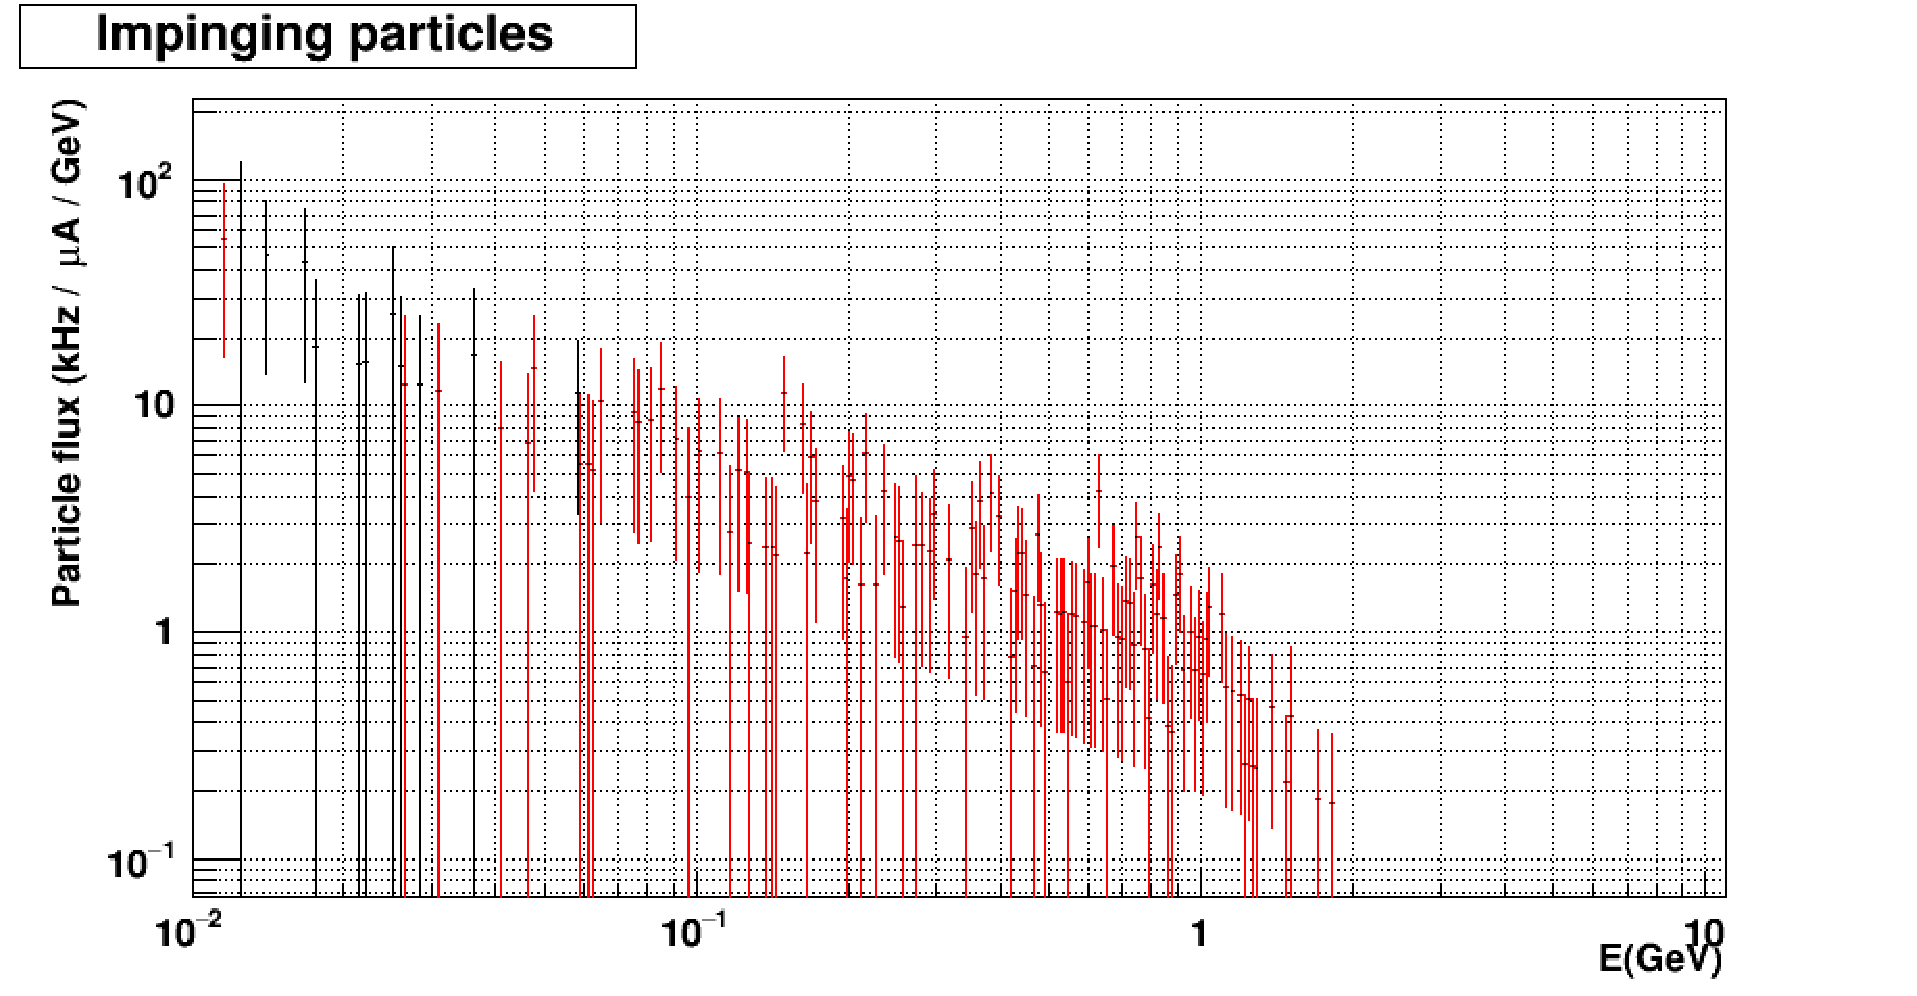
\includegraphics[width=10.0cm]{figs/fig19_crsB.pdf}
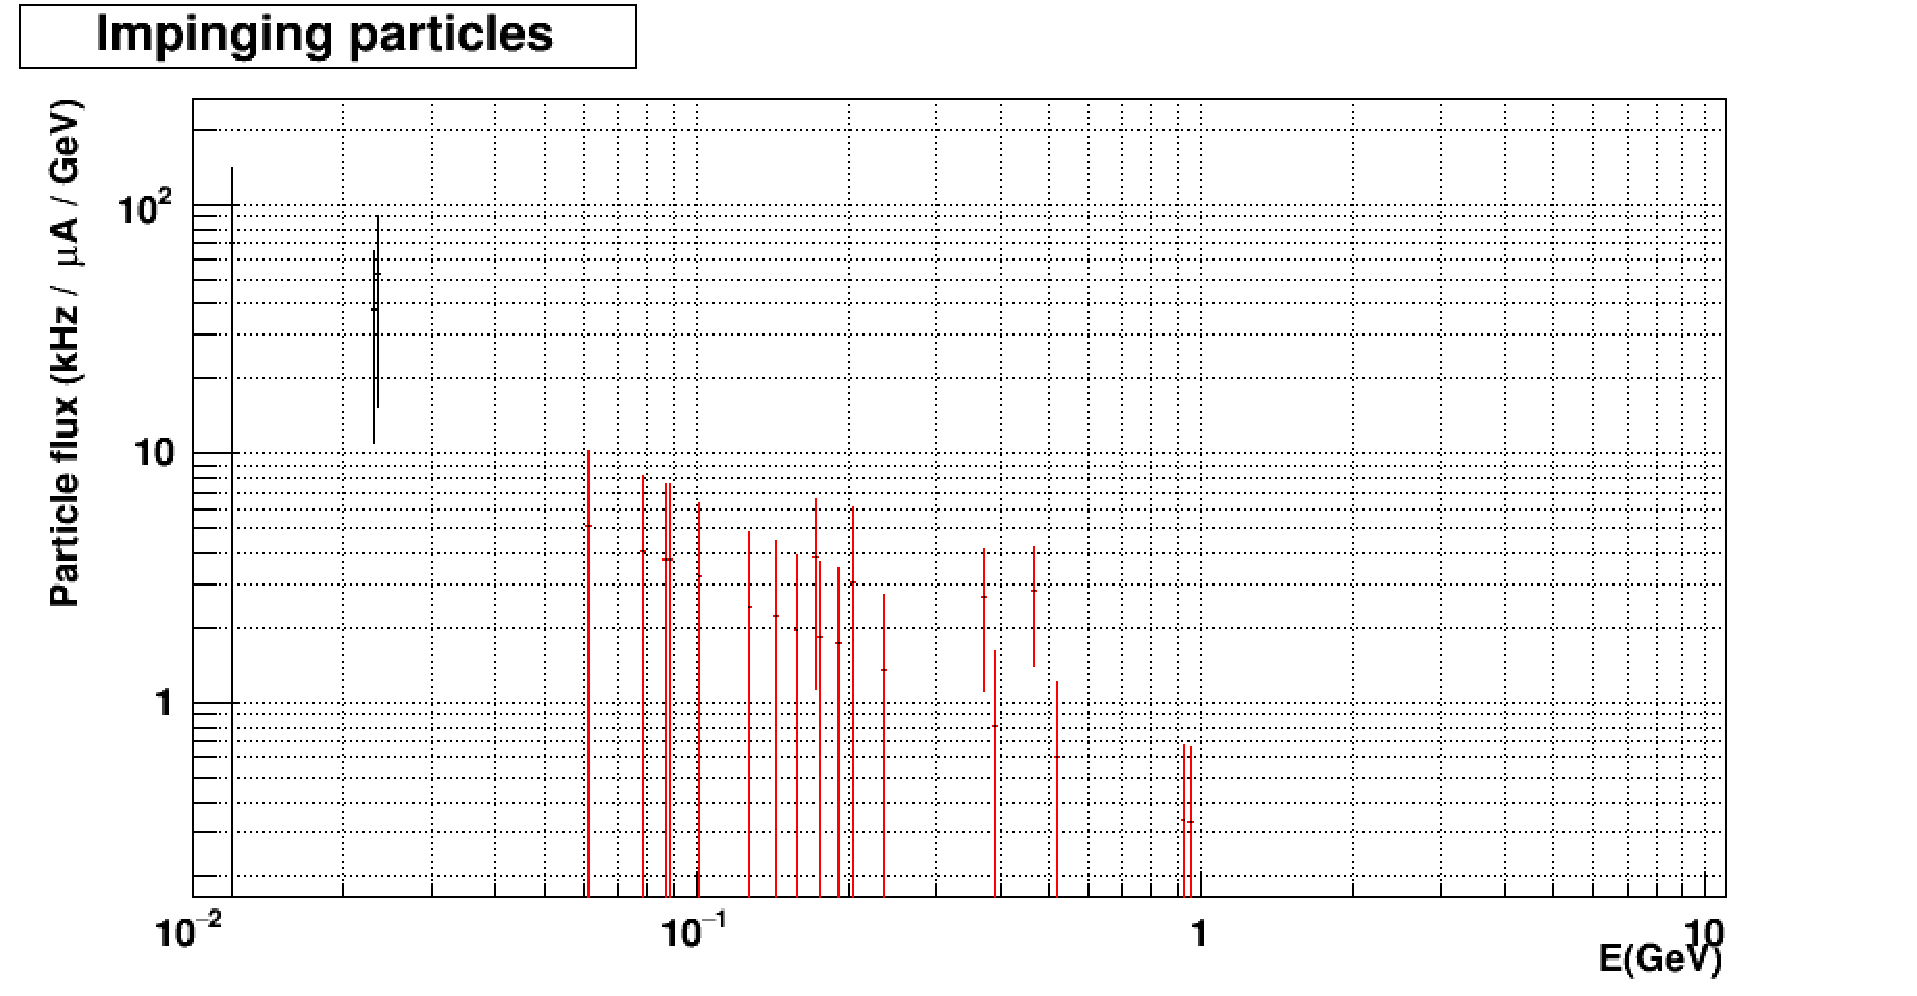
\includegraphics[width=10.0cm]{figs/fig19_crsC.pdf}
\caption {Fluence  of all particles (black) and muons only (red) hitting the CsI(Tl) crystal.
Plots refer to the crystal located in {\bf A} (top),  {\bf B} (middle), and {\bf C} (bottom).}
\label{fig:fluence-mAs}
\end{figure}

For a complete understanding of the low energy ($<$ MeV) background in the BDX-Hodo crystal, particles produced in the dump can not be tracked separately since some of them are produced along the way (e.g by energetic muons or neutrons in the proximity of the detector). On top of that, neutral particles (in particular low energy/thermal neutron) do not directly interact with the crystal but deposit a visible energy via secondary interactions (e.g. gamma from nuclear capture in the surrounding material) making hard, if not impossible,  to track back the background source. For all the above mentioned reasons we evaluated the background by running the  full FLUKA simulation of  11 GeV electrons interaction with the beam-dump recording  the deposited energy in BDX-Hodo crystal. 
Figure~\ref{fig:fluence-mAs} shows the fluence of all particles (black) and muons only (red) on the CsI(Tl) surface. As already noticed, the high energy range of the spectrum is saturated by muons. 
\begin{figure}[h!] 
\center
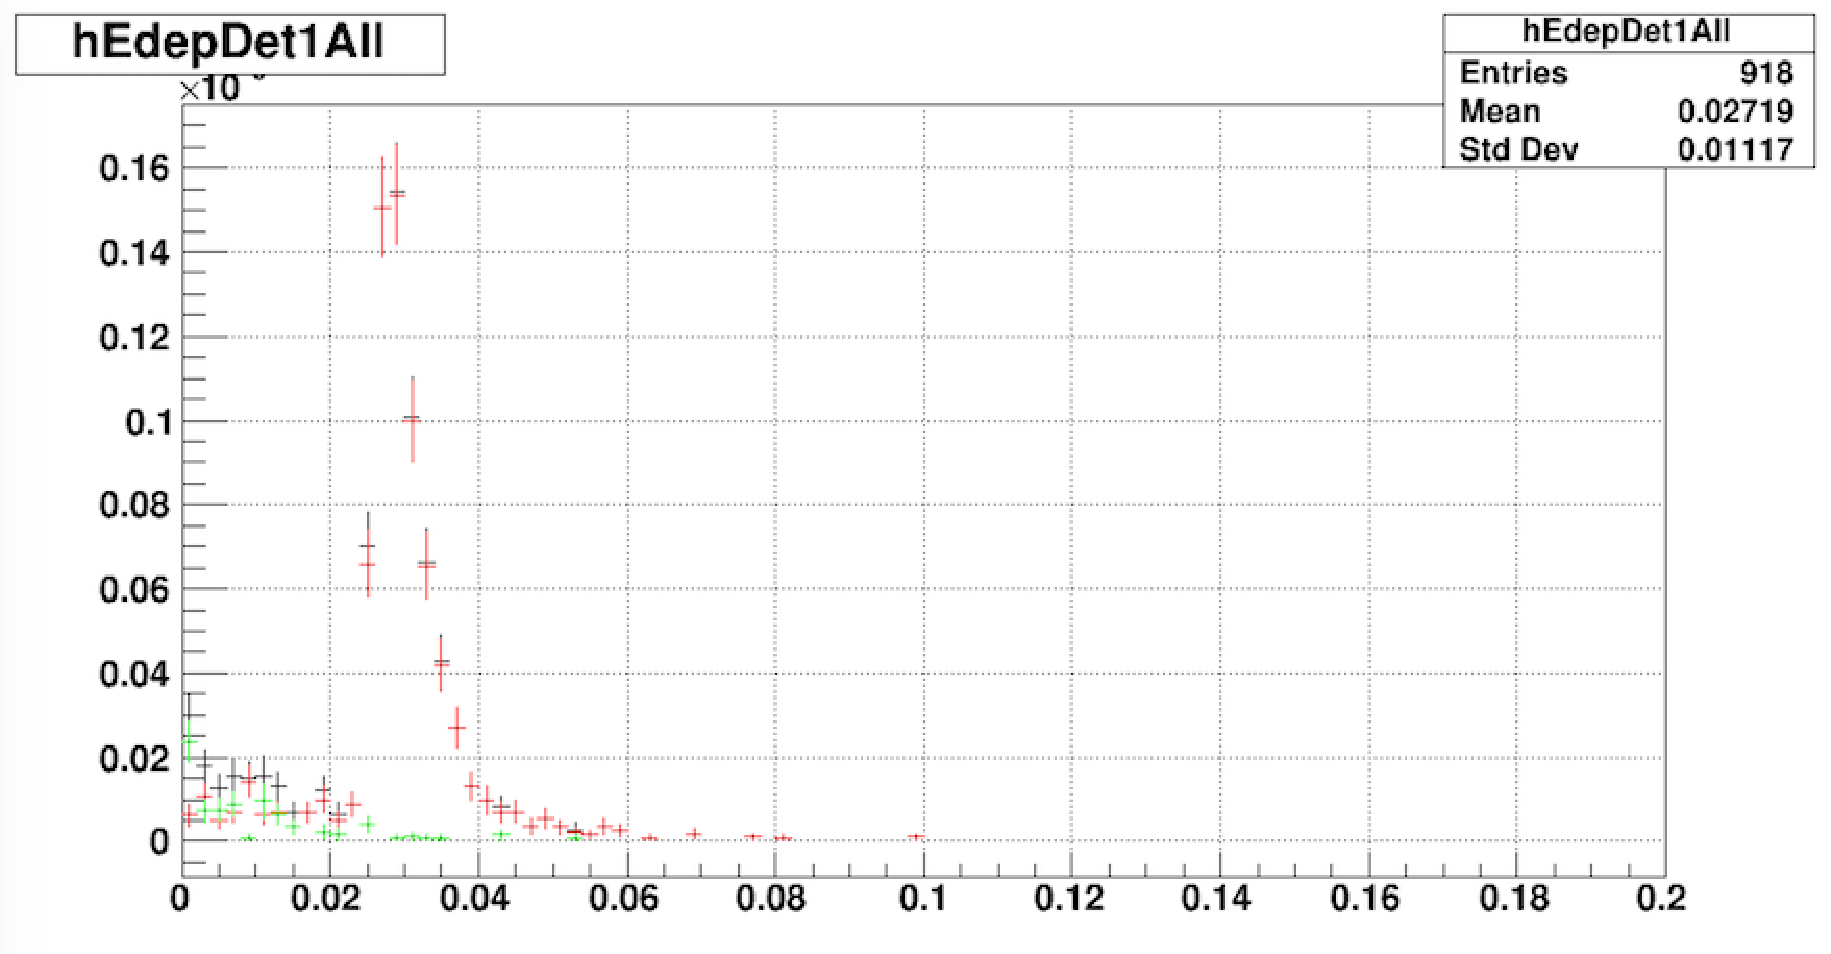
\includegraphics[width=12.0cm]{figs/Edep1.pdf}
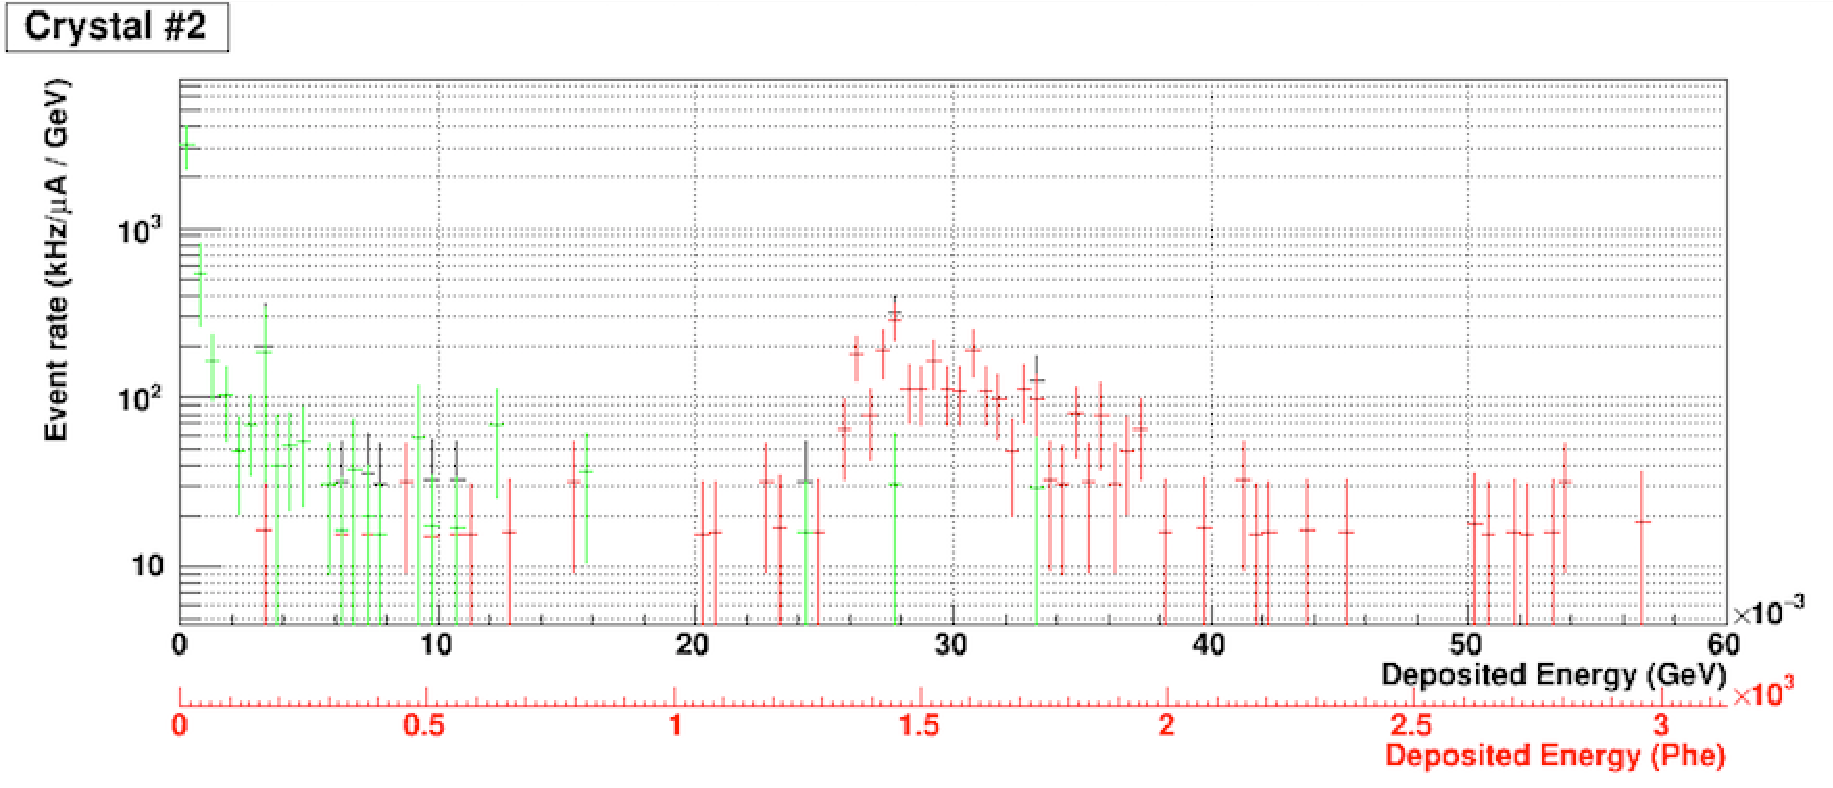
\includegraphics[width=12.0cm]{figs/Edep2.pdf} 
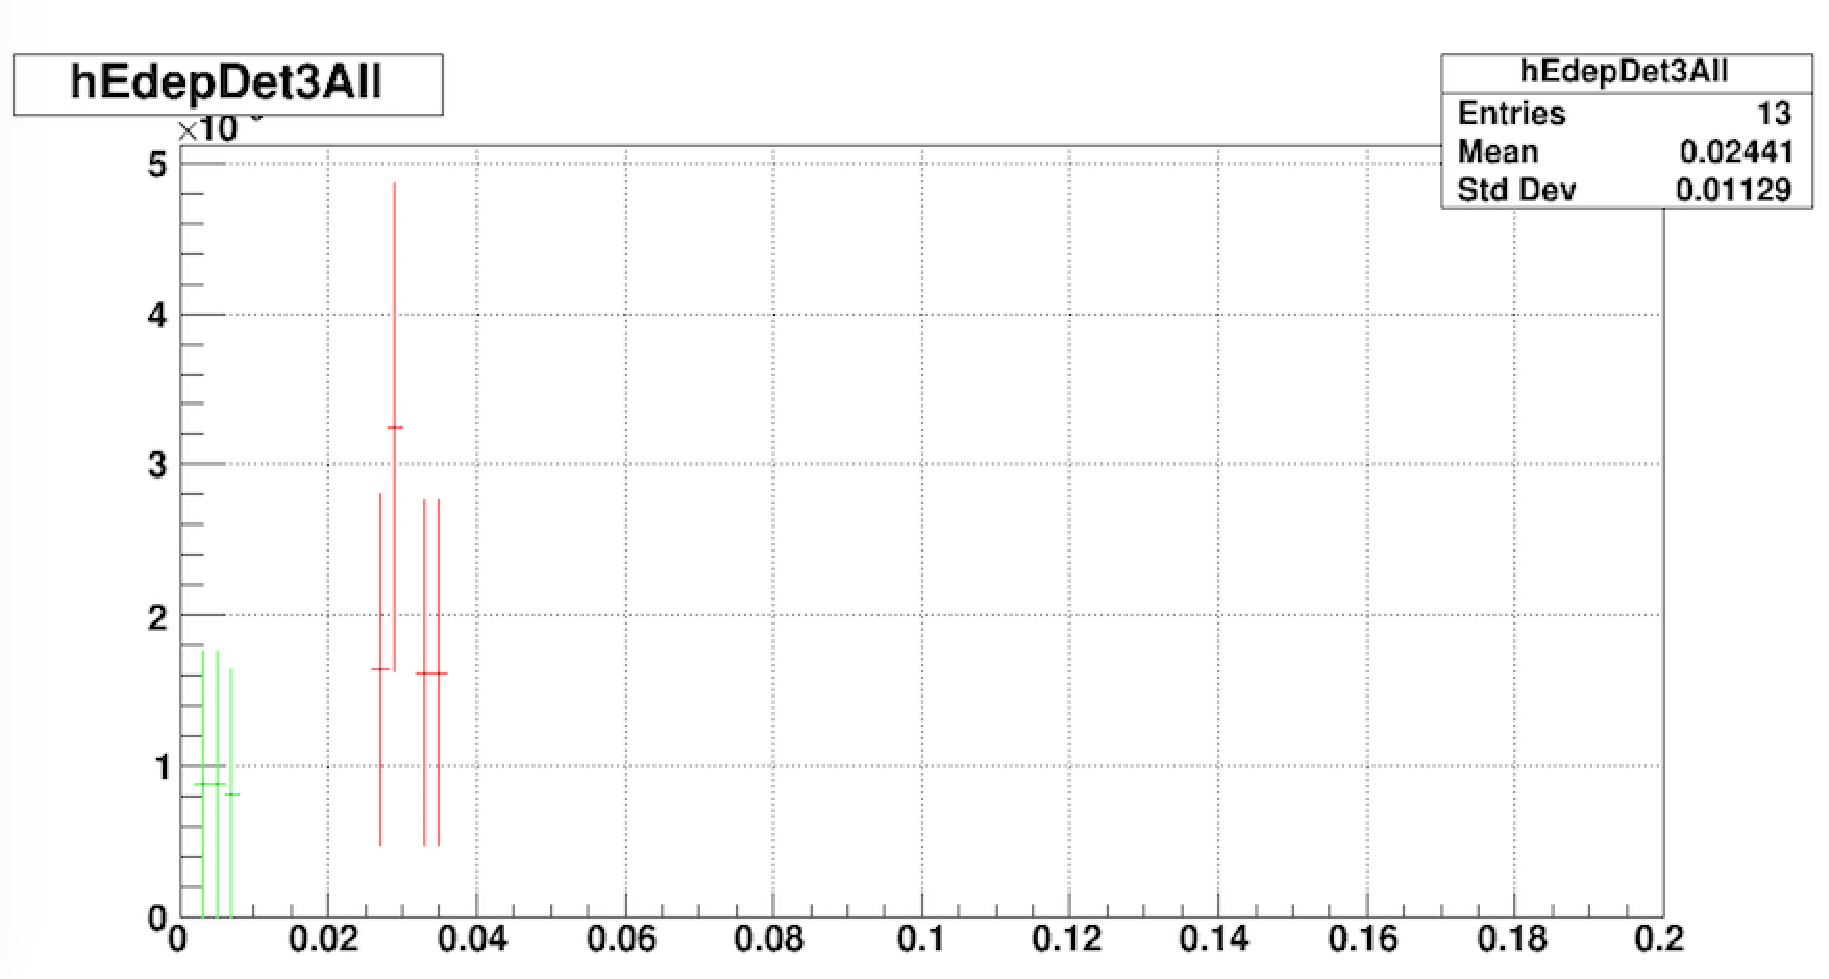
\includegraphics[width=12.0cm]{figs/Edep3.pdf}
\caption {Distribution of energy deposited in the CsI(Tl) crystal by all particles (black), muons only (red) and the rest (green). The three plots refer to the crystal located in {\bf A} (left),  {\bf B} (center), and {\bf C} (right).}
\label{fig:edep}
\end{figure}
Figure~\ref{fig:edep} shows the deposited energy in the CsI(Tl) crystal (located in the three  position of interest).  Muons (shown in red) almost saturate the highest energies (the MIP peak is clearly visible around E$_{Dep}$ = 32 MeV) while the contribution from other particles (neutrons) accumulates at low energies.
\begin{figure}[h!] 
\center
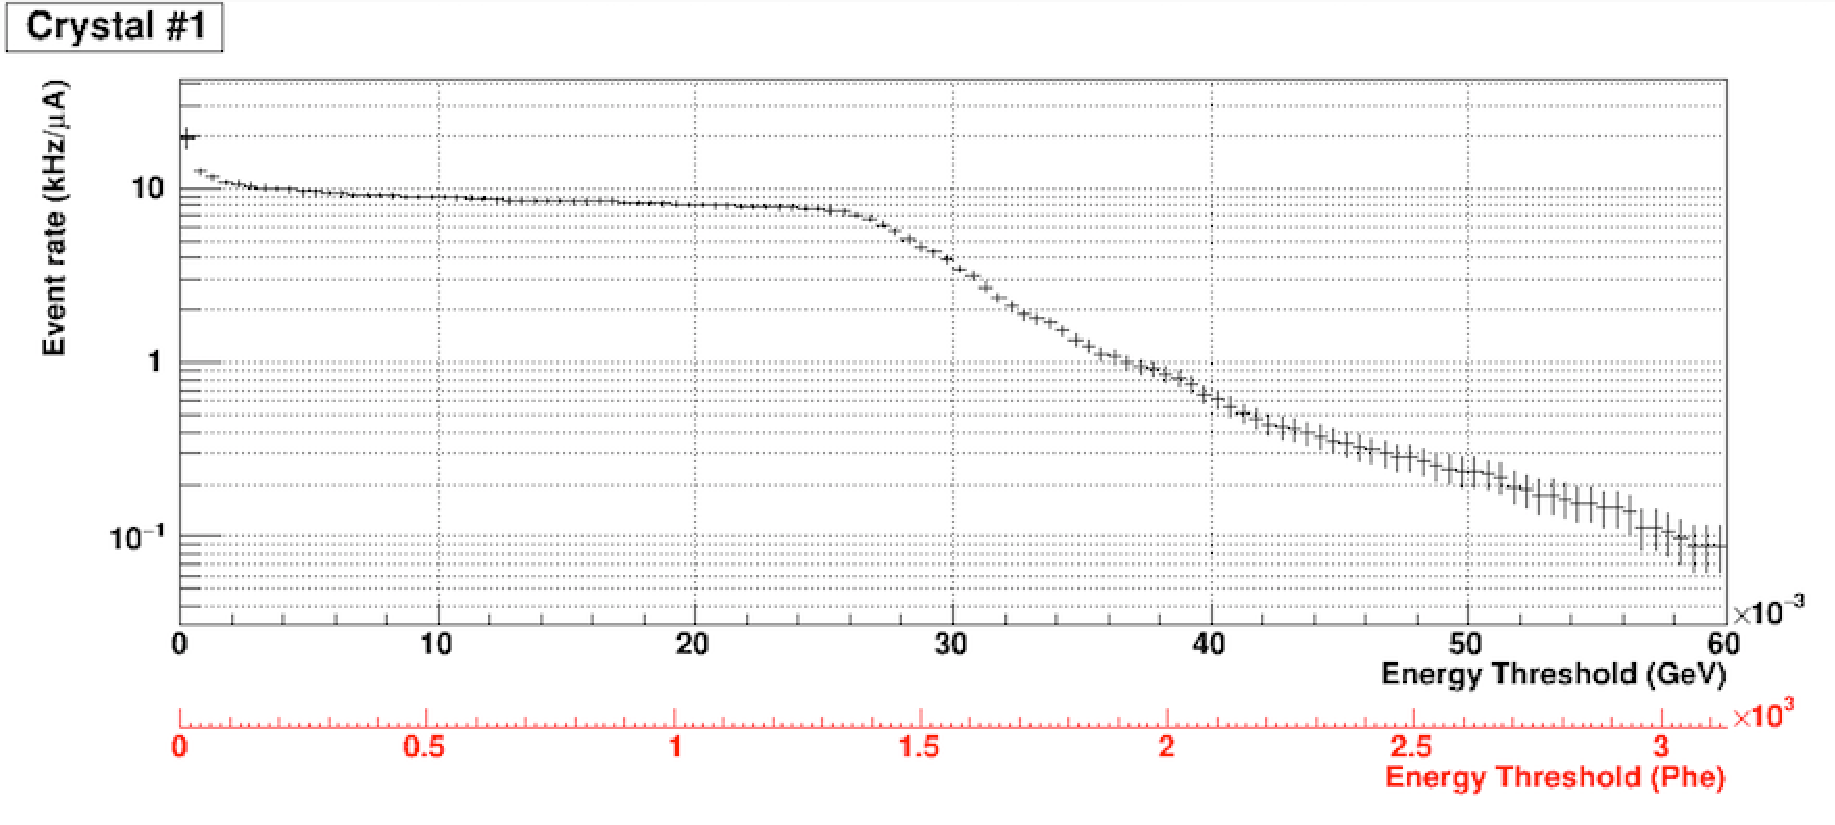
\includegraphics[width=12.0cm]{figs/int-rate-E1.pdf} 
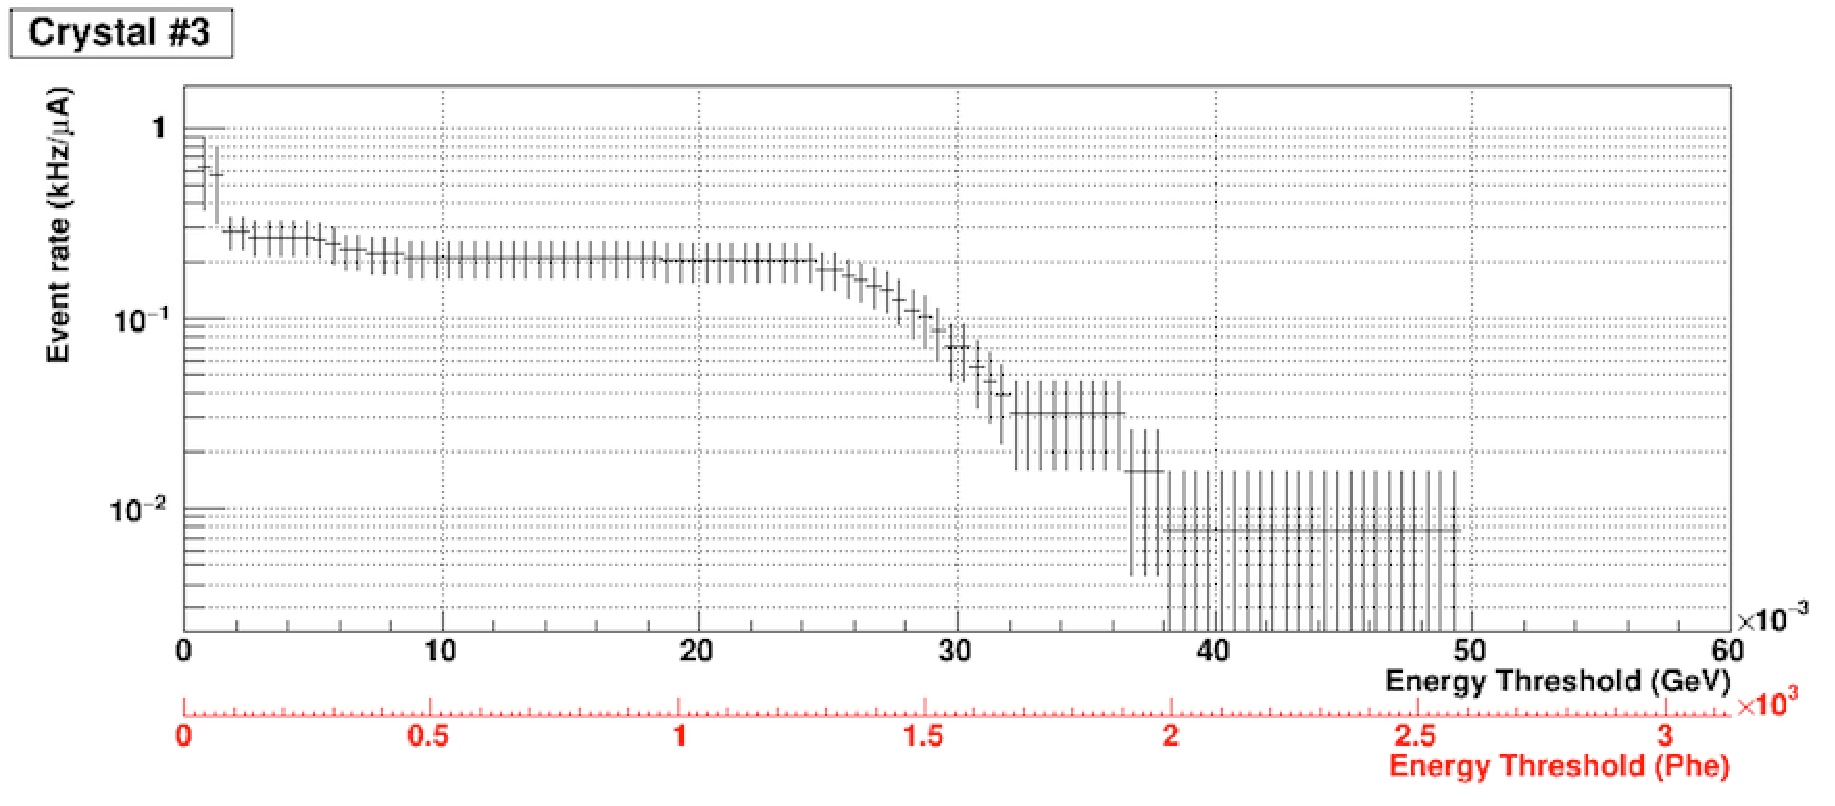
\includegraphics[width=12.0cm]{figs/int-rate-E2.pdf} 
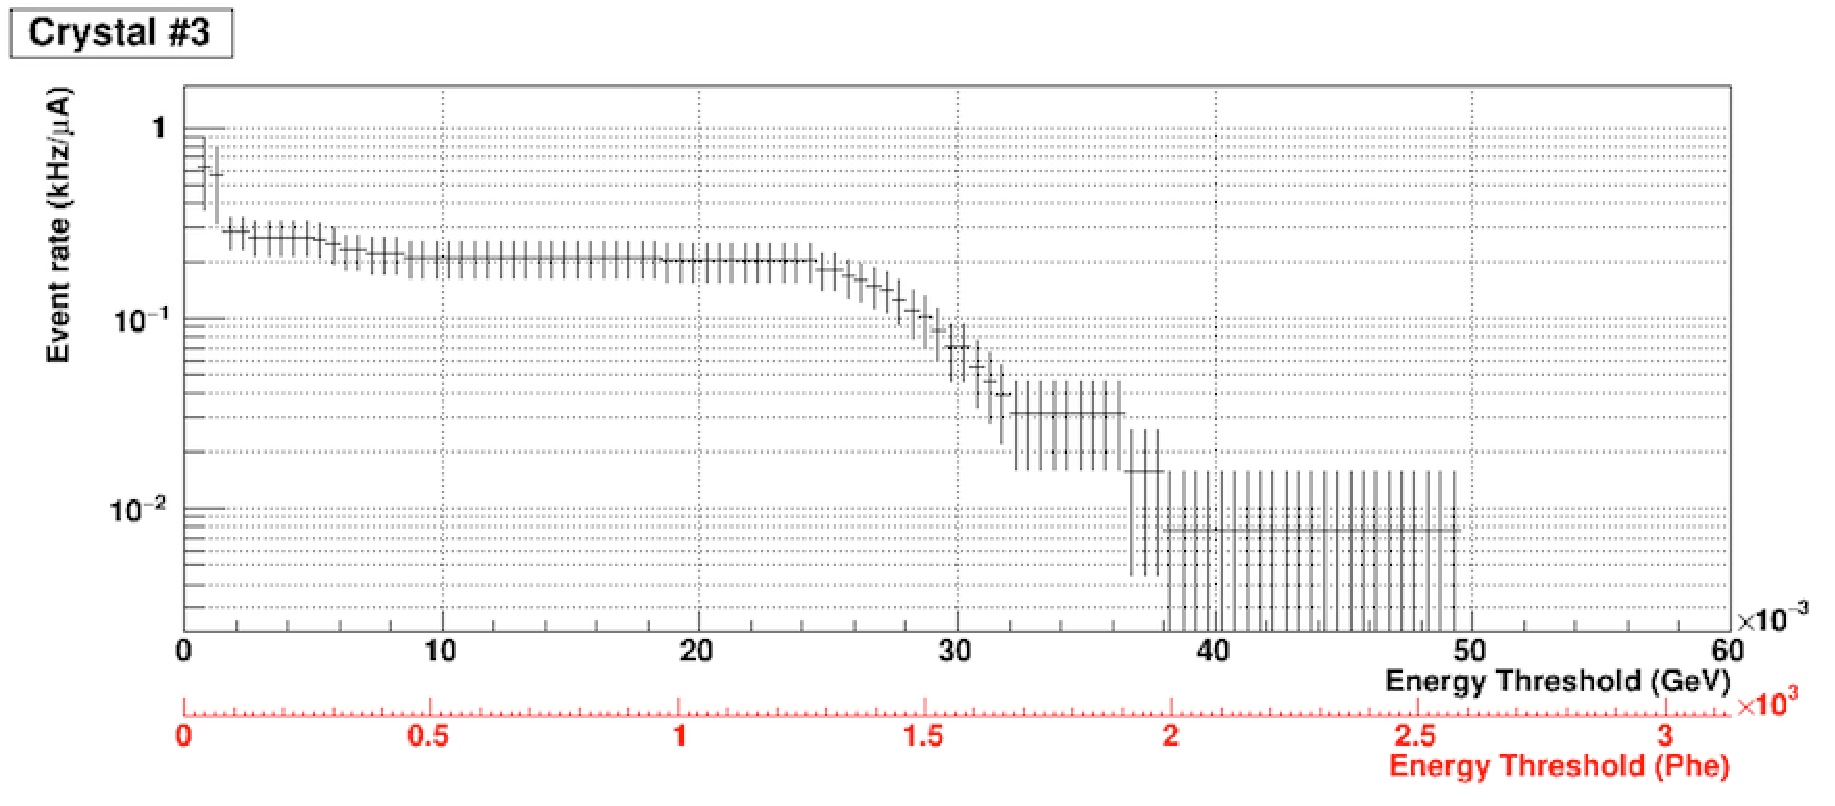
\includegraphics[width=12.0cm]{figs/int-rate-E3.pdf}
\caption {Crystal integrated rate as function of deposited energy.
Plots refer to the crystal located in {\bf A} (left),  {\bf B} (center), and {\bf C} (right).}
\label{fig:int-rates-E}
\end{figure}

The crystal  integrated rate is reported in Fig.~\ref{fig:int-rates-E}  as a function of the deposited energy (and detected photoelectrons). Considering that  the experiment only records events 
with a deposited energy in the crystal  larger than  1 MeV (25 pe), the expected rate is in the range of 10 kHz.
%It worth to notice that even a background rate in the range of 1 MHz does not represent an issue since the low energy deposited ($<$1 MeV) corresponds to signals of one/few photoelectrons spread over the entire scintillation time window ($\sim 1 \mu$s) making it not distinguishable from  other noise (e.g. SiPM dark current, preamplifier noise, ...).

\subsubsection{Cosmic background}
The cosmic muon background in the BDX-Hodo has been evaluated using GEMC. This is the same cosmic flux generator used in PR-16-001~\cite{bdx-proposal}. The muon energy spectrum has been divided in different ranges  and correctly weighted to estimate the full rate expected on the detector. Rates have been evaluated for CsI(Tl) crystal, Top scintillator,  and for the coincidence of the front/back scintillator with the crystal  to mimic the condition used to identify and account for beam-on muons. We assumed the same detection thresholds used in the other rate estimates (10 phe and 100 phe for scintillators and crystal respectively). Tab.~\ref{tab:cosmic} shows the results of this study. The cosmic rate is negligible (in every condition $<$ 1 Hz) well below the expected rate of muons from the electron beam / beam-dump interaction.

\begin{table}[htp]
\caption{Cosmic rate expected in different components of BDX-Hodo}
\begin{center}
\begin{tabular}{|c|c|c|c|}
\hline
Energy range  (GeV) & Rate$_{Crystal}$  (Hz)&  Rate$_{Top\,Scintillator} $(Hz) & Rate$_{Coincidence}$ (Hz) \\
\hline\hline
 0.2 - 2  & 0.01 &  0.02 & 0\\
 \hline
 2 - 10  & 0.2 &  0.25 & 0.01\\
 \hline
 10 - 100  & 0.35 &  0.4 & 0.01\\
\hline\hline
Cosmic muon rate  & 0.56 &  0.67 & 0.02 \\
\hline\hline
\end{tabular}
\end{center}
\label{tab:cosmic}
\end{table}%

\subsection{Test configuration and practical details}
Practical details (drilling technology, costs and schedule) and a work plan for the proposed test configuration  are reported in the Appendix.

\subsection{Summary}
We simulated the interaction of a 11 GeV electron beam with the Hall-A beam-dump studying the   radiation field in the beam-dump vault and   $\sim$20 m downstream
 in the area of  the new underground  facility required by the BDX experiment. Two different  simulation tools (GEMC and FLUKA) were used. For some locations, results were compared with JLab Radiological Control Group estimates. 
Here are the main outcome:
\begin{itemize}
\item{our results are consistent with what obtained by RadCon;}
\item{we confirm that only (high energy) muons and (mainly  thermal/low energy) neutrons propagates trough the beam-dump vault concrete walls  and dirt reaching the region of intereset; }
\item{no sizeable flux was found outdoor in the closest locations above-the-ground;}
\item{for energy greater than 100 MeV muon and neutron flux estimated with FLUKA and GEMC well match;}
\item{for energy lower than 100 MeV  FLUKA (using the biasing technique)  resulted more efficient in run-time. }
\end{itemize}
To validate MC tools and gain confidence in the beam-on background shielding optimization  for the  BDX experiment we propose to measure the muon flux in the region where the new underground facility will be located. 
Here below is the proposed experimental set up and the expected results:
\begin{itemize}
\item{muons produced in the dump can be accessed by playcing a  detector downstream at the beam-line depth;}
\item{a detector  (BDX-Hodo) based on one CsI(Tl) crystal from  BDX ECal, sandwiched between layers of scintillator counters  will be specifically built for this measurement;}
\item{ two wells equipped by  10' pipes will be drilled  25.2 m and 28 m downstream of the beam-dump and the BDX-Hodo detector lowered in a pipe to cross the beam axes;}
\item{rates of beam-on muons measured by BDX-Hodo are expected  to be sizeable for  a beam current of 10 $\mu A$ ($\sim$3 kHz and $\sim$20 kHz in the two locations respectively);}
\item{given the count rates reported above, this measurement could be done  with a variety of beam current (1 - 100 $\mu A$ ) making the test fully parasitic wrt the Hall-A plans;}
\item{this measurement was found to be insensitive to the cosmic muon background and other backgrounds (mainly) neutrons generated in the dump; }
\item{the use of a BDX CsI(Tl) crystal will allow to prove the proposed technology in a background-rich environment worst than what expected in the BDX experiment\footnote{The BDX experiment foresees  an optimised shilding that will drastically reduce  any possible background.}; }
\item{once the pipes will be installed, tests will run for about a week, parasitically  to  any 11 GeV 1-100 $\mu$A, Hall-A run;} 
This  test, measuring the muon flux (absolute and relative) in different location in Z (distance from the dump) and Y (vertical) will address the concern expressed by PAC44 report about the beam-on background in the BDX experiment.
\end{itemize}

